% Appendix C

\chapter{Screenshots der Anwendung}
\label{Screenshots_der_Anwendung}

\section{Screenshots des Prototyps}

\begin{figure}[!h]
	\centering
		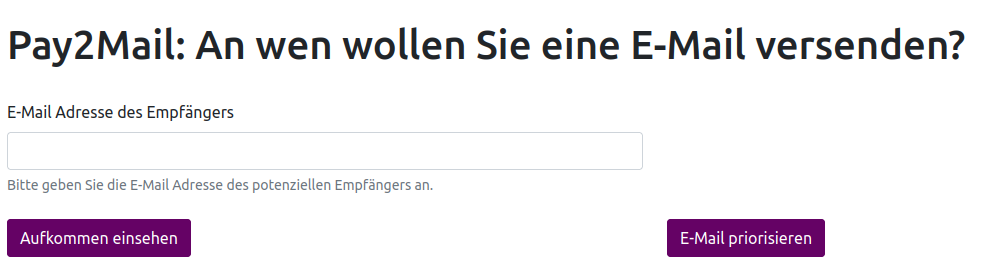
\includegraphics[width=1.2\textwidth]{Figures/send_overview.png}
	\caption{Screenshot: Absenderübersicht im Prototyp}
	\label{fig:screenshot_send/overview}
\end{figure}

\begin{figure}[!h]
	\centering
		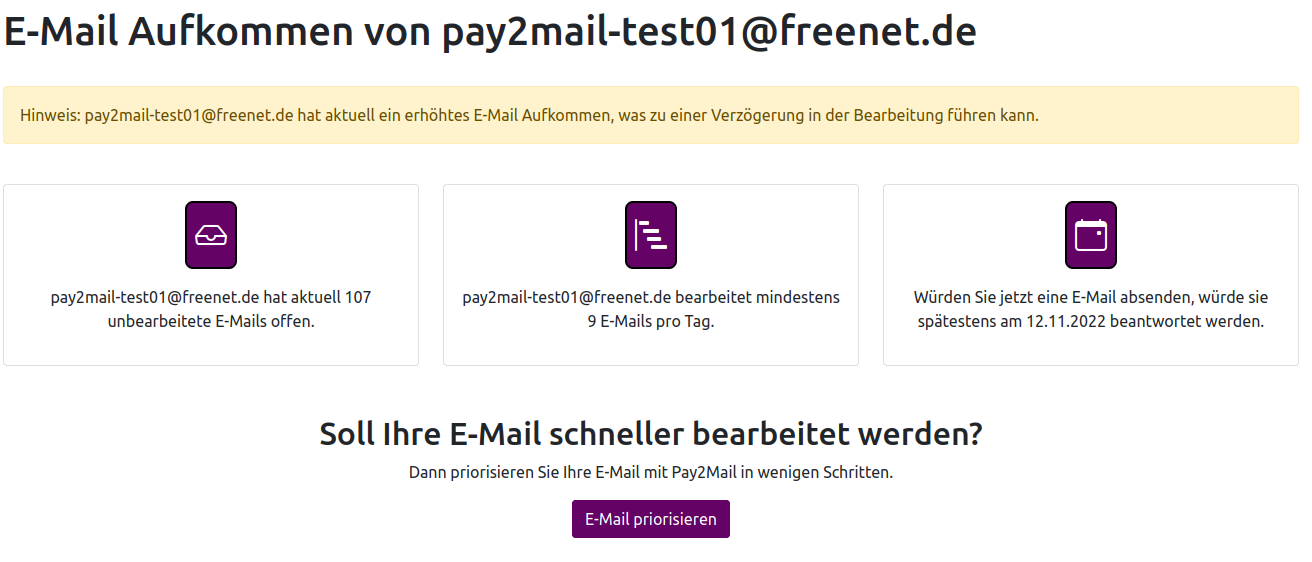
\includegraphics[width=1.2\textwidth]{Figures/send_capacity.png}
	\caption{Screenshot: E-Mail Aufkommen des Empfängers im Prototyp}
	\label{fig:screenshot_send/capacity}
\end{figure}

\begin{figure}[!h]
	\centering
		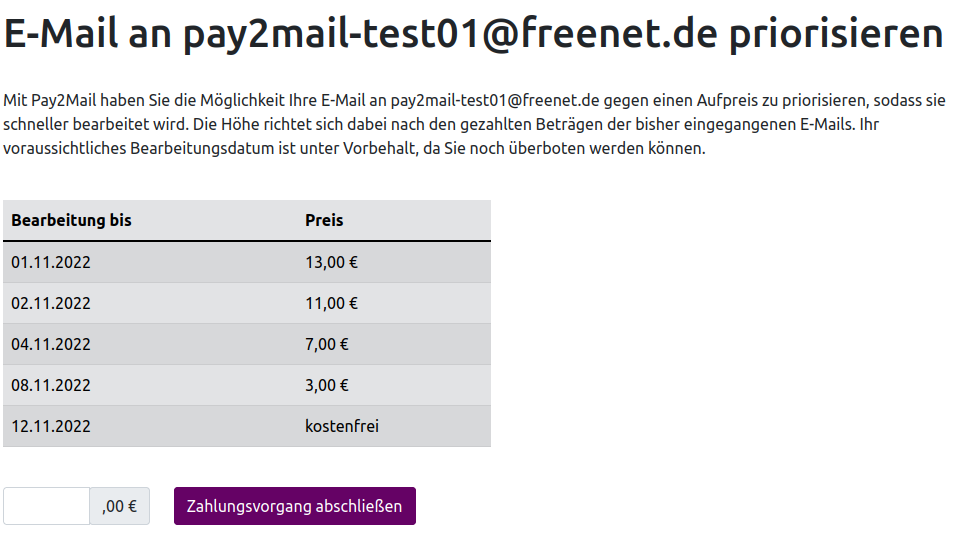
\includegraphics[width=1\textwidth]{Figures/send_priority.png}
	\caption{Screenshot: Priorisierungsmöglichkeiten für Empfänger im Prototyp}
	\label{fig:screenshot_send/priority}
\end{figure}

\newpage
\section{Screenshots des ersten Arbeitspaketes}

\begin{figure}[!h]
	\centering
		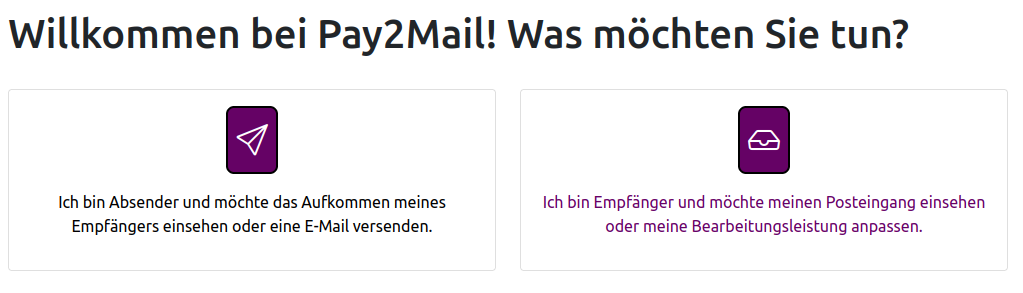
\includegraphics[width=1\textwidth]{Figures/overview.png}
	\caption{Screenshot: Startseite zur Auswahl von Absenderfrontend oder Empfängerfrontend}
	\label{fig:screenshot_overview}
\end{figure}

\newpage
\section{Screenshots des zweiten Arbeitspaketes}

\begin{figure}[!h]
	\centering
		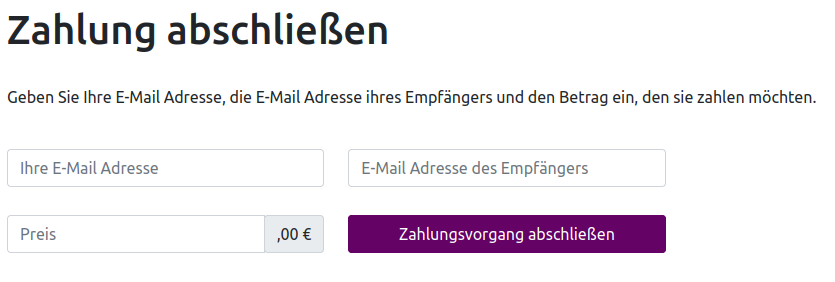
\includegraphics[width=1\textwidth]{Figures/send_priority_new.png}
	\caption{Screenshot: Formular zur Priorisierung einer E-Mail}
	\label{fig:screenshot_send/priority_new}
\end{figure}

\begin{figure}[!h]
	\centering
		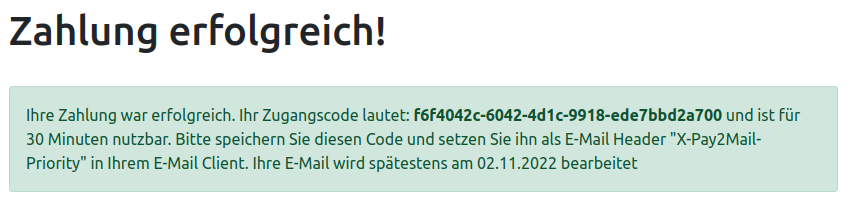
\includegraphics[width=1\textwidth]{Figures/send_priority_show.png}
	\caption{Screenshot: Anzeige eines erstellten Gegenwert-Headers}
	\label{fig:screenshot_send/priority_show}
\end{figure}

\newpage
\section{Screenshots des dritten Arbeitspaketes}

\begin{figure}[!h]
	\centering
		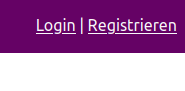
\includegraphics[width=0.25\textwidth]{Figures/header1.png}
	\caption{Screenshot: Oberer rechter Teil des Headers bei ausgeloggtem Nutzer}
	\label{fig:screenshot_header1}
\end{figure}

\begin{figure}[!h]
	\centering
		
\includegraphics[width=0.5\textwidth]{Figures/header2.png}
	\caption{Screenshot: Oberer rechter Teil des Headers bei eingeloggtem Nutzer}
	\label{fig:screenshot_header2}
\end{figure}

\begin{figure}[!h]
	\centering
		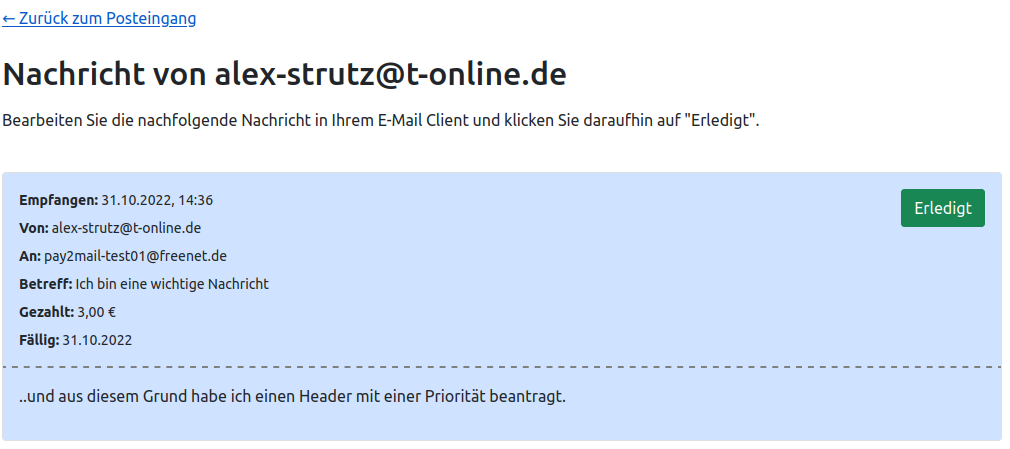
\includegraphics[width=1.1\textwidth]{Figures/message.png}
	\caption{Screenshot: Einzelansicht einer Nachricht für Empfänger}
	\label{fig:screenshot_message}
\end{figure}

\begin{figure}[!h]
	\centering
		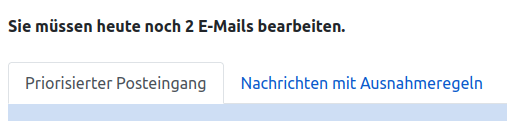
\includegraphics[width=0.6\textwidth]{Figures/tab.png}
	\caption{Screenshot: \texttt{Tab}-Komponente mit Möglichkeit zum Wechseln der Posteingangstabellen}
	\label{fig:screenshot_inbox2}
\end{figure}

\begin{figure}[!h]
	\centering
		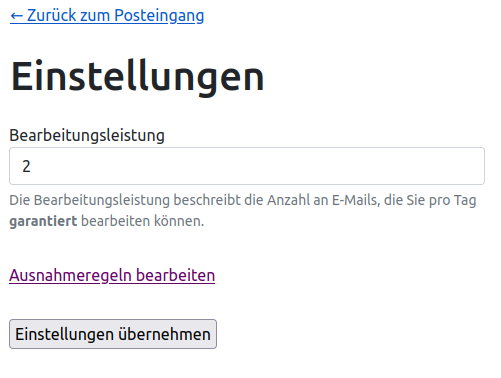
\includegraphics[width=0.75\textwidth]{Figures/recipients.png}
	\caption{Screenshot: Anpassung der Bearbeitungsleistung durch den Empfänger}
	\label{fig:screenshot_recipients}
\end{figure}

\begin{figure}[!h]
	\centering
		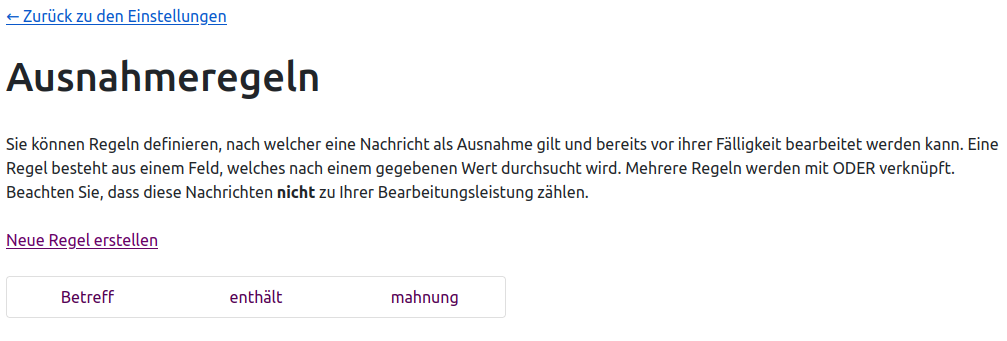
\includegraphics[width=1.1\textwidth]{Figures/rules1.png}
	\caption{Screenshot: Auflistung der definierten Regeln eines Empfängers}
	\label{fig:screenshot_rules1}
\end{figure}

\begin{figure}[!h]
	\centering
		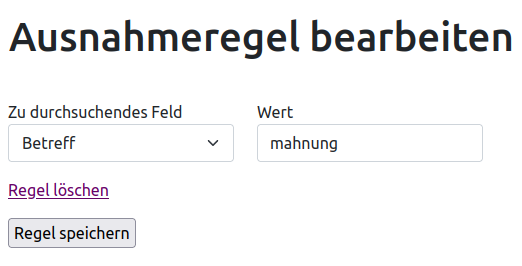
\includegraphics[width=0.75\textwidth]{Figures/rules2.png}
	\caption{Screenshot: Bearbeitung einer Regel durch den Empfänger}
	\label{fig:screenshot_rules2}
\end{figure}

\begin{figure}[!h]
	\centering
		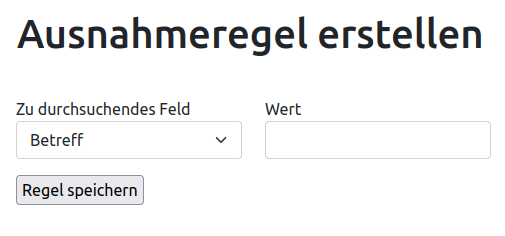
\includegraphics[width=0.75\textwidth]{Figures/rules3.png}
	\caption{Screenshot: Erstellung einer neuen Regel durch den Empfänger}
	\label{fig:screenshot_rules3}
\end{figure}

